\section{Другое}

\subsection{Типы ОС}

Однопрограммные пакетные обработчики --- в памяти хранится одна программа, но она считана из пакета.

Мультипрограммные пакетные обработкичи --- в памяти хранится несколько программ, считанных из пакета. Выполняются программы от начала и до конца --- неопределённое время ожидания.

Системы разделения времени --- процессорное время квантуется (очев., что системы разделения времени мультизадачные).

Наши компьютеры мультипрограммные и мультизадачные (одновременно выполняется несколько процессов; в однопроцессорных системах достигается засчёт быстрого переключения между задачами; в мультипроцессорных --- задачи фактически могут выполняться параллельно на разных процессорах).

\subsection{Прерывания}

Операциями ввода-вывода управляет устройство; процессор от этого освобождён.
Появилась необходимость информаировать процессор о завершении операций ввода-вывода --- возникла система пререываний:
\begin{enumerate}
    \item системные вызовы (программные прерывания),
    \item исключения,
    \item аппаратные прерывания:
    \begin{itemize}
        \item прерывания от системного таймера (единственное периодическое),
        \item прерывания от внешних устройств (информируют процессор о завершении операций ввода-вывода),
        \item прерывания от действий оператора (KeyboardInterrupt, ...).
    \end{itemize}
\end{enumerate}

Процессор и память связаны локальной шиной, называемой локальной шиной памяти.

Процессор памяти не имеет и постоянно обменивается данными с оперативной памятью.
Регистры --- неотъемлемая часть процессора, это не память.

Процессор --- регистры, управляемые передачей данных.
В процессоре тоже есть микропрограммное управление.
Процессор --- тоже программно управляемое устройство.

Принцип хранимой программы (основной принцип фон Неймана) --- процессор может выполнять программу, которая хранится в ОЗУ; и данные, и команды хранятся в одной и той же память; обращение к командам и данным выполняется только по адресу (расположены в памяти в последовательных адресах).

В состав процессора входит PC (IP в Intel) --- всегда содержит адреса команд, которые надо считать из памяти (адрес следующей команды).

Настраивается на начальный адрес сначала, считывает следующую команду, увеличивает IP на размер следующей команды --- базовый принцип работы вычислительных машин.

Внешние устройства адресуются также, как ячейки памяти.
В компьютере всё адресуется.
К внешним устройствам процессор обращается по адресу, но такой адрес называется портом. Порт --- это адрес.

Если процессору надо обратиться к внешнему устройству, он устанавливает порт; дальше в зависимости от ввода/вывода; в зависимости от устройства, либо устанавливает, либо получает данные из шины данных.

В 3-м поколении ЭВМ была реализована идея распараллеливания функций.
Функции управления внешними устройствами от процессора были переданы следующим устройствам:
\begin{itemize}
    \item селекторы и мультиплексоры (в канальной архитектуре),
    \item контроллер (в шинной архитектуре); если в составе внешнего устройства --- контроллер, если в составе материнской платы --- адаптер.
\end{itemize}

Контроллер по шине данных от процессора получает команды, которые управляют операциями ввода-вывода --- появилась система прерываний.

Существует три типа прерываний (что бы Microsoft ни говорил):
\begin{enumerate}
    \item Системные вызовы (вызов системы) --- так называемые программные прерывания --- программа прерывается, чтобы перейти на управление системного вызова --- кода ядра.
    \item Исключения --- ошибки системы, связанные с разными событиями в системе; ZeroDivisionError --- самая базовая. Разрядность в компах ограничена, нельзя представить $\infty$, поэтому ZeroDivisionError.
    \item Аппаратные прерывания (*Interrupt) --- аппаратное прерывание возникает в системе в результате завершения выполнения внешними устройствами операций ввода-вывода. Управляет не процессор, а контроллер или каналы --- необходимо проинформировать процессор о том, что операция ввода-вывода завершена. То есть, аппаратные прерывания формируются контроллером прерываний, когда внешнее устройство завершает операции ввода-вывода.
\end{enumerate}

\begin{figure}[H]
	\centering
	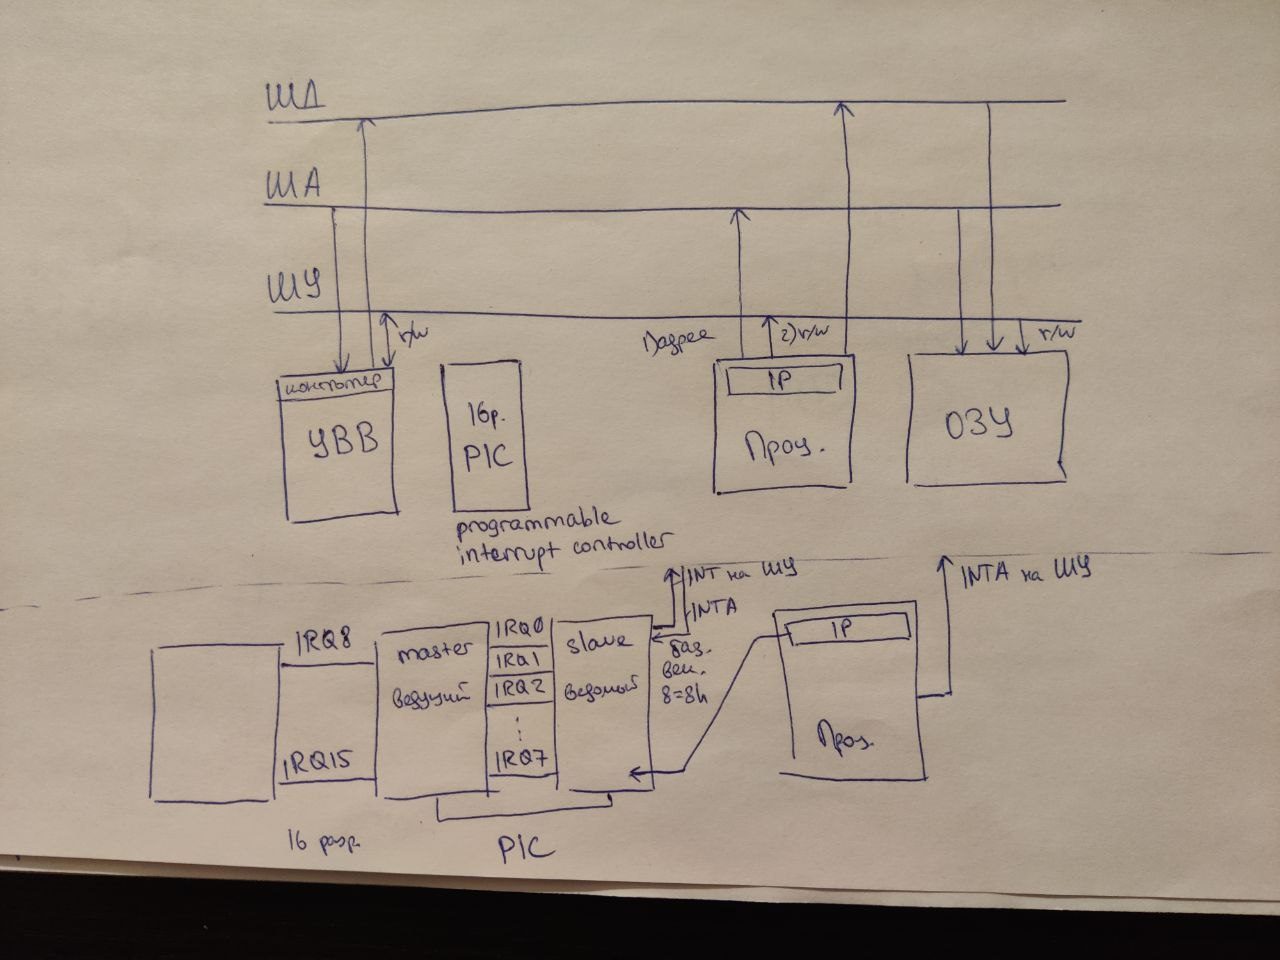
\includegraphics[width=\textwidth]{img/tables/06.jpg}
	% \caption{}
	% \label{fig:}
\end{figure}

На линию поступает сигнал прерывания от контроллера внешних устройств.

IRQ0 --- туда приходит прерывание от системного таймера, так называемый <<тик>>.
В реальном режиме формируется 18.2 раза в секунду.
Единственное периодическое прерывание в системе.
Все остальные прерывания от внешних устройств возникают в случайным момент времени.
Даже используются для генерации случайных чисел.

IRQ1 --- туда приходят прерывания клавиатуры (разъём ПС/2); клавиатура ноутбука --- IRQ1, мышь --- IRQ12.

Когда на линию IRQ приходит сигнал прерывания от внешнего устройства; если этот сигнал прерывания замаскирован (разрешён), контроллер выставляет на шину управления сигнал INT.

\begin{figure}[H]
	\centering
	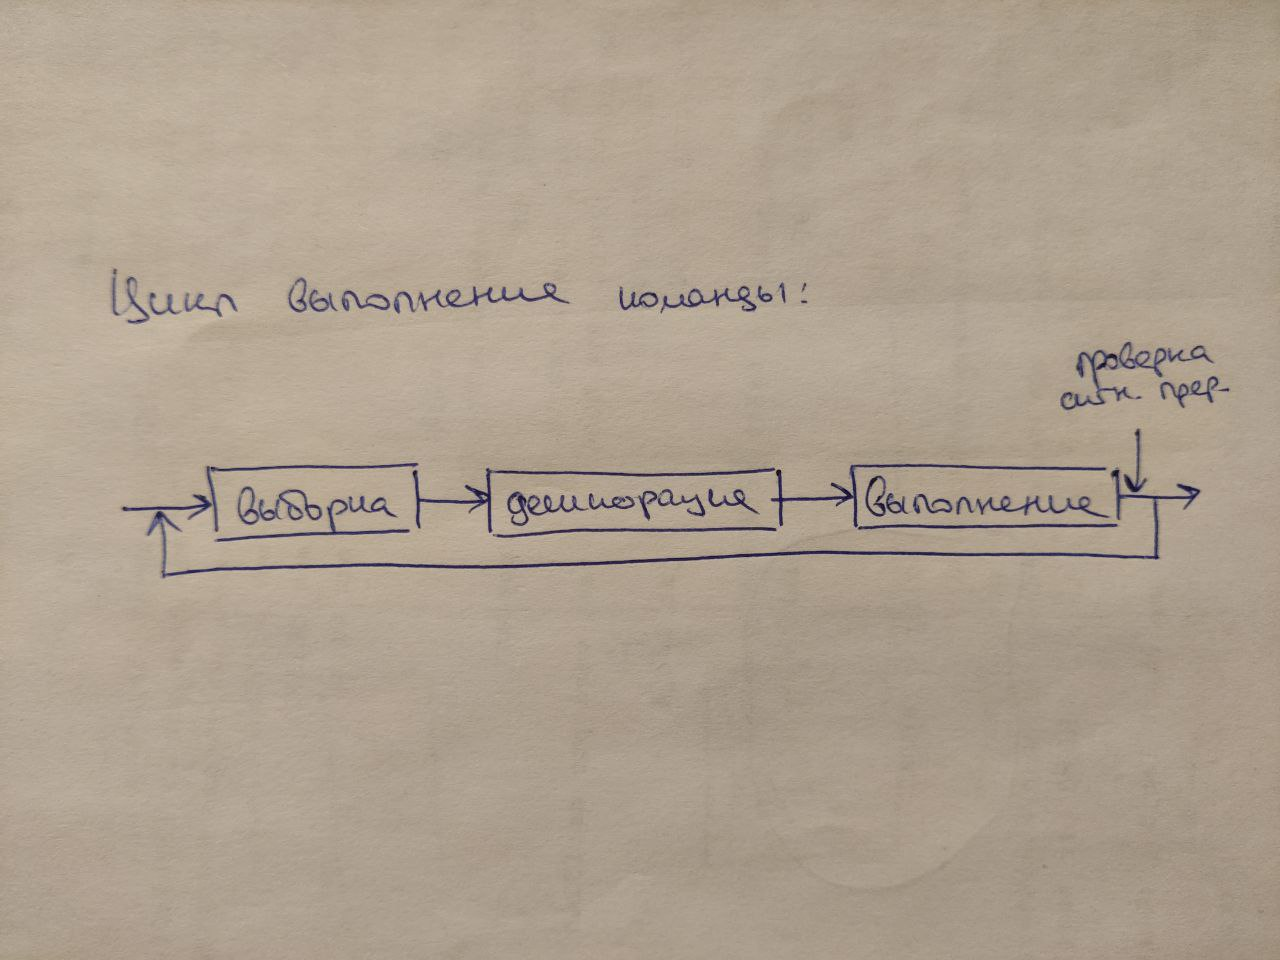
\includegraphics[width=\textwidth]{img/tables/07.jpg}
	% \caption{Цикл выполнения команды}
	% \label{fig:}
\end{figure}

Процессор проверяет наличие сигнала прерывания на выделенной ножке.
Если сигнал прерывания пришёл, то процессор отсылает ответный сигнал --- INTA.
Потом выставляет на вектор прерываний (вектор прерываний --- базовый вектор + номер линии IRQ).
В реальном режиме (16 р.) базовый вектор контроллера равен 8.
8 + 0 = 8; отсюда INT 8h название.

Вектор прерываний (ВП) по шине данных поступает в процессор.
Процессор по полученному вектору в реальном режиме обращается к таблице векторов прерываний (расположена в первом 1 КБ, начиная с 0).

Сам контроллер прерываний тоже адресуется, тоже через порт и по шине данных на контроллер посылается маска прерывания.

Тик приходит на линию IRQ0 контроллера прерываний и приводит к вызову обработчика прерывания от системного таймера.

\subsection{Диаграмма состояний процесса}

\subsubsection{Стадии}

\begin{figure}[H]
	\centering
	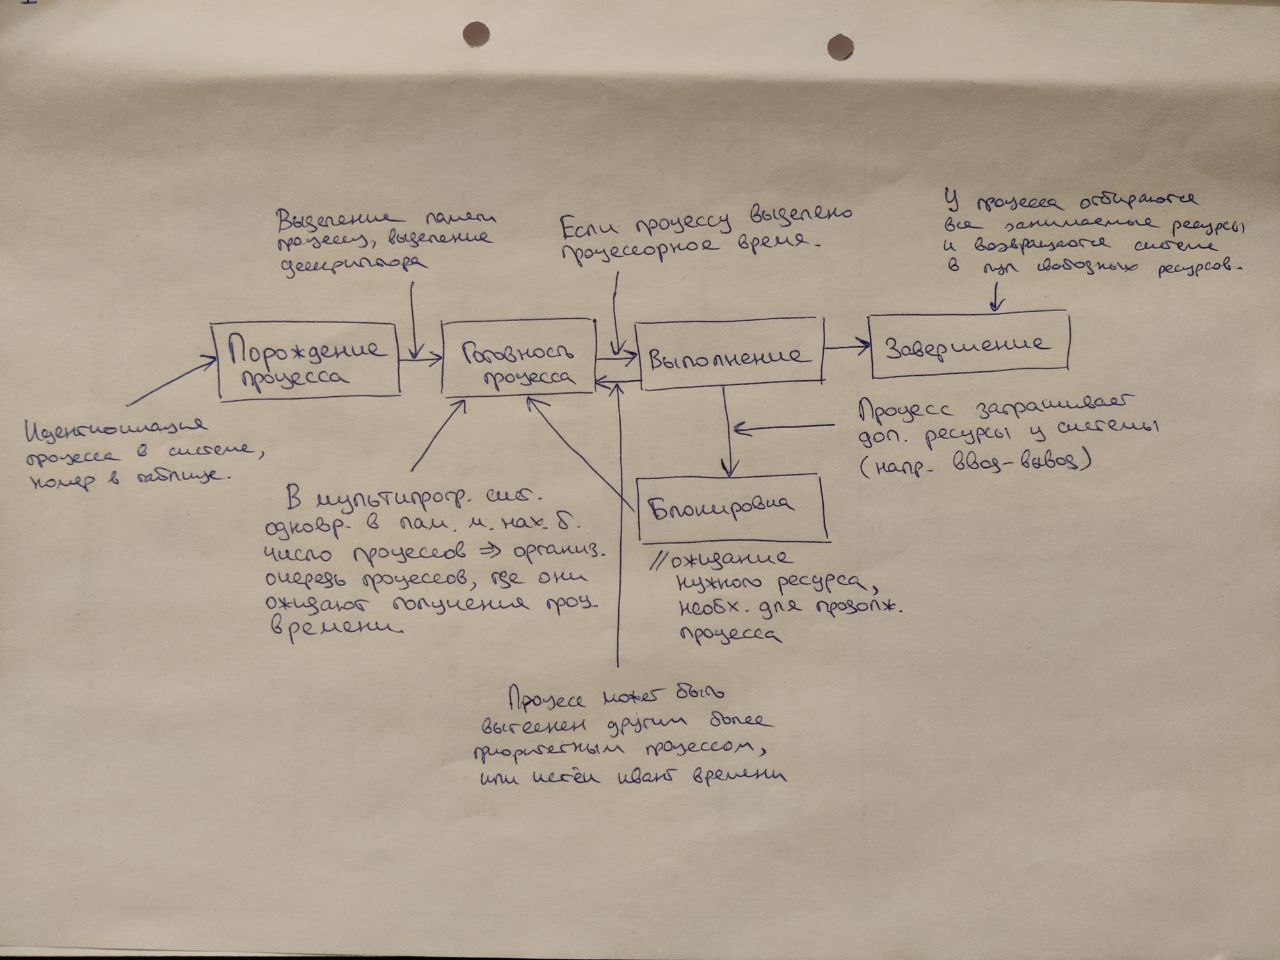
\includegraphics[width=\textwidth]{img/tables/01.jpg}
	% \caption{}
	% \label{fig:}
\end{figure}

\begin{enumerate}
    \item Идентификация процесса. Ни одна программа не может работать с неопределёнными значениями; для этого задаём имя и типы переменных --- это и есть идентификация переменных. Система также не может работать непонятно с чем --- должна идентифицировать процесс. В системе выполняется большое число процессов --- существуют средства описания процессов. В современном программировании этими средствами являются структуры (структуры появились в C).
    \item Описание дескриптора процесса (дескриптор --- описатель, структура, предназначенная для описания процесса). Существует поле, отражающее текущее состояние процесса; в этой структуре находится указатель на другую структуру, в частности, на структуру, предназначенную для управления памятью. Процессор может выполнять только программы, находящиеся в памяти.
    \item Система выделяет процессу память. Дескриптор должен содержать информацию о выделенной процессу памяти --- это означает, что программа загружена в физическую память; псоле этого программа может начать выполняться.
\end{enumerate}

Планирование --- постановка процессов в очередь (очев., что процессорное время получит процесс, находящийся первым в очереди) по каким-то принципам.

Диспечеризация --- выделение процессорного времени.

% TODO: до семафоров, где spin_lock, test_and_set, до этого

\section{Взаимоисключение}

Для того, чтобы не происходило race conditions, к разделяемым переменным (в общем случае, к разделяемым ресурсам) должен обеспечиваться монопольный доступ --- если один процесс обратился к разделяемой переменной, никакой другой процесс к ней обратиться не может, пока тот процесс не освободит переменную.
Монопольный доступ обеспечивается средствами взаимоисключения.

\section{Семафоры}
